% SPMAC extended abstract (Selecciones Matematicas) -- DRAFT
% Source of every number: docs/RESULTS.md, docs/NOISE_ROBUSTNESS.md,
% results/hard_benchmark.json, results/noise_robustness.md (repo at commit ae3edd4).
% TODO before submission:
%   * port to the official SPMAC / Selecciones Matematicas template (page limit 3-6 pp.);
%   * author list, affiliations, corresponding e-mail (collaborators: J. Lincovil, E. Cayun);
%   * complete the reference for the original multiview descriptor;
%   * archive the code (e.g. Zenodo DOI) and update the availability statement;
%   * check the MSC codes.
\documentclass[11pt,a4paper]{article}
\usepackage[utf8]{inputenc}
\usepackage[T1]{fontenc}
\usepackage[margin=2.3cm]{geometry}
\usepackage{amsmath,amssymb}
\usepackage{graphicx}
\usepackage{booktabs}
\usepackage[hidelinks]{hyperref}
\graphicspath{{../../results/figures/}}

\title{Do persistent-homology descriptors detect coherent structures better
than classical diagnostics?\\ A structure-only benchmark in two-dimensional
turbulence}
\author{[Author names -- TODO]\\
\small [Affiliations -- TODO]\quad \texttt{[corresponding e-mail -- TODO]}}
\date{}

\begin{document}
\maketitle

\begin{abstract}
Persistent homology is increasingly proposed for identifying coherent
structures and flow regimes in geophysical fluids, but most evaluations use
regimes that spectral or one-point statistics already separate. We build a
\emph{structure-only} benchmark that removes this shortcut. We take 240
snapshots of forced two-dimensional turbulence ($256^2$, three forcing scales,
24 independent trajectories) and pair each with an IAAFT surrogate that has
the same power spectrum and value histogram, so that only the Fourier phases,
i.e.\ the spatial structure, differ. Spectrum and histogram classifiers score
at chance (0.50). Under trajectory-grouped cross-validation, a
topological--spectral multiview descriptor reaches 98.9\% accuracy, and richer
vectorizations reach 99--100\%. Classical diagnostics (Okubo--Weiss,
vorticity-gradient and increment statistics) reach 97--100\%, however, and no
topological configuration beats their concatenation by the pre-specified
margin of 0.05 on any of the six clean-field tasks. Under strong observation noise a multi-scale
filtration keeps 99\% accuracy, but the same classical diagnostics on the same
Gaussian pyramid do equally well. On this benchmark persistent homology
detects coherent structure, but at parity with standard diagnostics, not
better.
\end{abstract}

\noindent\textbf{Keywords:} persistent homology; two-dimensional turbulence;
coherent structures; surrogate data; IAAFT; Okubo--Weiss parameter.\\
\textbf{MSC 2020:} 55N31, 76F65, 76M22, 62H30. % TODO: check

\section{Introduction}

Coherent vortices, filaments and fronts control transport and mixing in
geophysical flows, and detecting them is a classical problem, usually
addressed with kinematic criteria such as the Okubo--Weiss parameter
\cite{okubo1970,weiss1991,isern2006}. Topological data analysis offers an
alternative. Persistent homology summarizes the connectivity of sub- and
superlevel sets of a field at all thresholds, is stable under perturbations
\cite{edelsbrunner2010,cohensteiner2007}, and has been applied to Kolmogorov
flow and Rayleigh--B\'enard convection \cite{kramar2016}.

Such descriptors are hard to evaluate fairly. Flow regimes that differ in
Reynolds number or forcing scale also differ in their energy spectrum, so
high accuracy can come from spectral information alone. In a preliminary run
of our own pipeline on such regimes, a single spectral slope and raw
down-sampled pixels both classified the regimes almost perfectly. That
accuracy says nothing about structure.

This note tests whether a topological--spectral multiview descriptor,
originally developed for discriminating neural architectures
\cite{multiview}, detects coherent structure better than classical
diagnostics. Our contributions are:
\begin{enumerate}
\item a structure-only benchmark in which spectrum and one-point statistics
  are blind by construction, with explicit leak detectors;
\item a comparison, under trajectory-grouped cross-validation and paired
  bootstrap confidence intervals, of the descriptor, its views and richer
  vectorizations against classical coherent-structure diagnostics;
\item the finding that topology achieves parity, not superiority, including
  under pre-registered degradations of the fields;
\item a round-off pitfall in field standardization that can silently create
  spurious separability.
\end{enumerate}

\section{A structure-only benchmark}

\paragraph{Coherent fields.} We solve the forced-dissipative vorticity
equation on $[0,2\pi)^2$,
\begin{equation}
\partial_t\omega + \mathbf{u}\cdot\nabla\omega
  = \nu\nabla^2\omega - \mu\,\omega + A\,k_f\cos(k_f y),
\qquad \nabla^2\psi=-\omega,\quad \mathbf{u}=(\partial_y\psi,-\partial_x\psi),
\end{equation}
with a pseudo-spectral method ($256^2$ modes, 2/3-rule dealiasing), an
integrating-factor fourth-order Runge--Kutta scheme ($\Delta t=0.005$), viscosity
$\nu=10^{-3}$ and linear (Ekman) drag $\mu=0.1$. The forcing scales are
$k_f\in\{4,8,16\}$ with amplitudes $A\in\{0.6,1.0,1.5\}$, chosen so that every
regime is turbulent rather than laminar Kolmogorov flow. For each $k_f$ we run 8
trajectories from independent random initial conditions and keep 10 snapshots
per trajectory, 3 time units apart, after 25 time units of spin-up. The flows
are statistically stationary after about 15 time units. Each field is
standardized to zero mean and unit variance, which gives 240 coherent fields.

\paragraph{Surrogates.} For every field $x$ we generate an iterative
amplitude-adjusted Fourier transform (IAAFT) surrogate
\cite{schreiber1996,venema2006}. It starts from a random permutation of
$x$ and alternates two steps: (a) impose the target Fourier amplitudes
$|\hat x(\mathbf{k})|$ while keeping the current phases, with Hermitian
symmetry enforced; (b) rank-order the result onto the sorted values of $x$.
We run 100 iterations and return the output of step (a). Its Fourier
amplitudes then match those of $x$ to a relative error of $4\times10^{-16}$, including the
exactly-zero dealiased modes, and its histogram matches to $0.023\,\sigma$ on
average, with differences only in the tails. This is the conservative variant:
any residual leak favours the one-point baselines, not the descriptor. The
histogram-exact variant (output of step (b)) gives identical conclusions.
Coherent fields and surrogates (Fig.~\ref{fig:fields}) therefore share every
spectral and one-point statistic and differ only in phase, i.e.\ in coherent
spatial structure, as in classical surrogate tests for nonlinearity
\cite{theiler1992}. Coherent field versus surrogate is the binary
\emph{primary task} (480 fields). We also use a 6-class task (forcing scale
$\times$ coherent/surrogate) and the binary task within each forcing scale.

\begin{figure}[t]
\centering
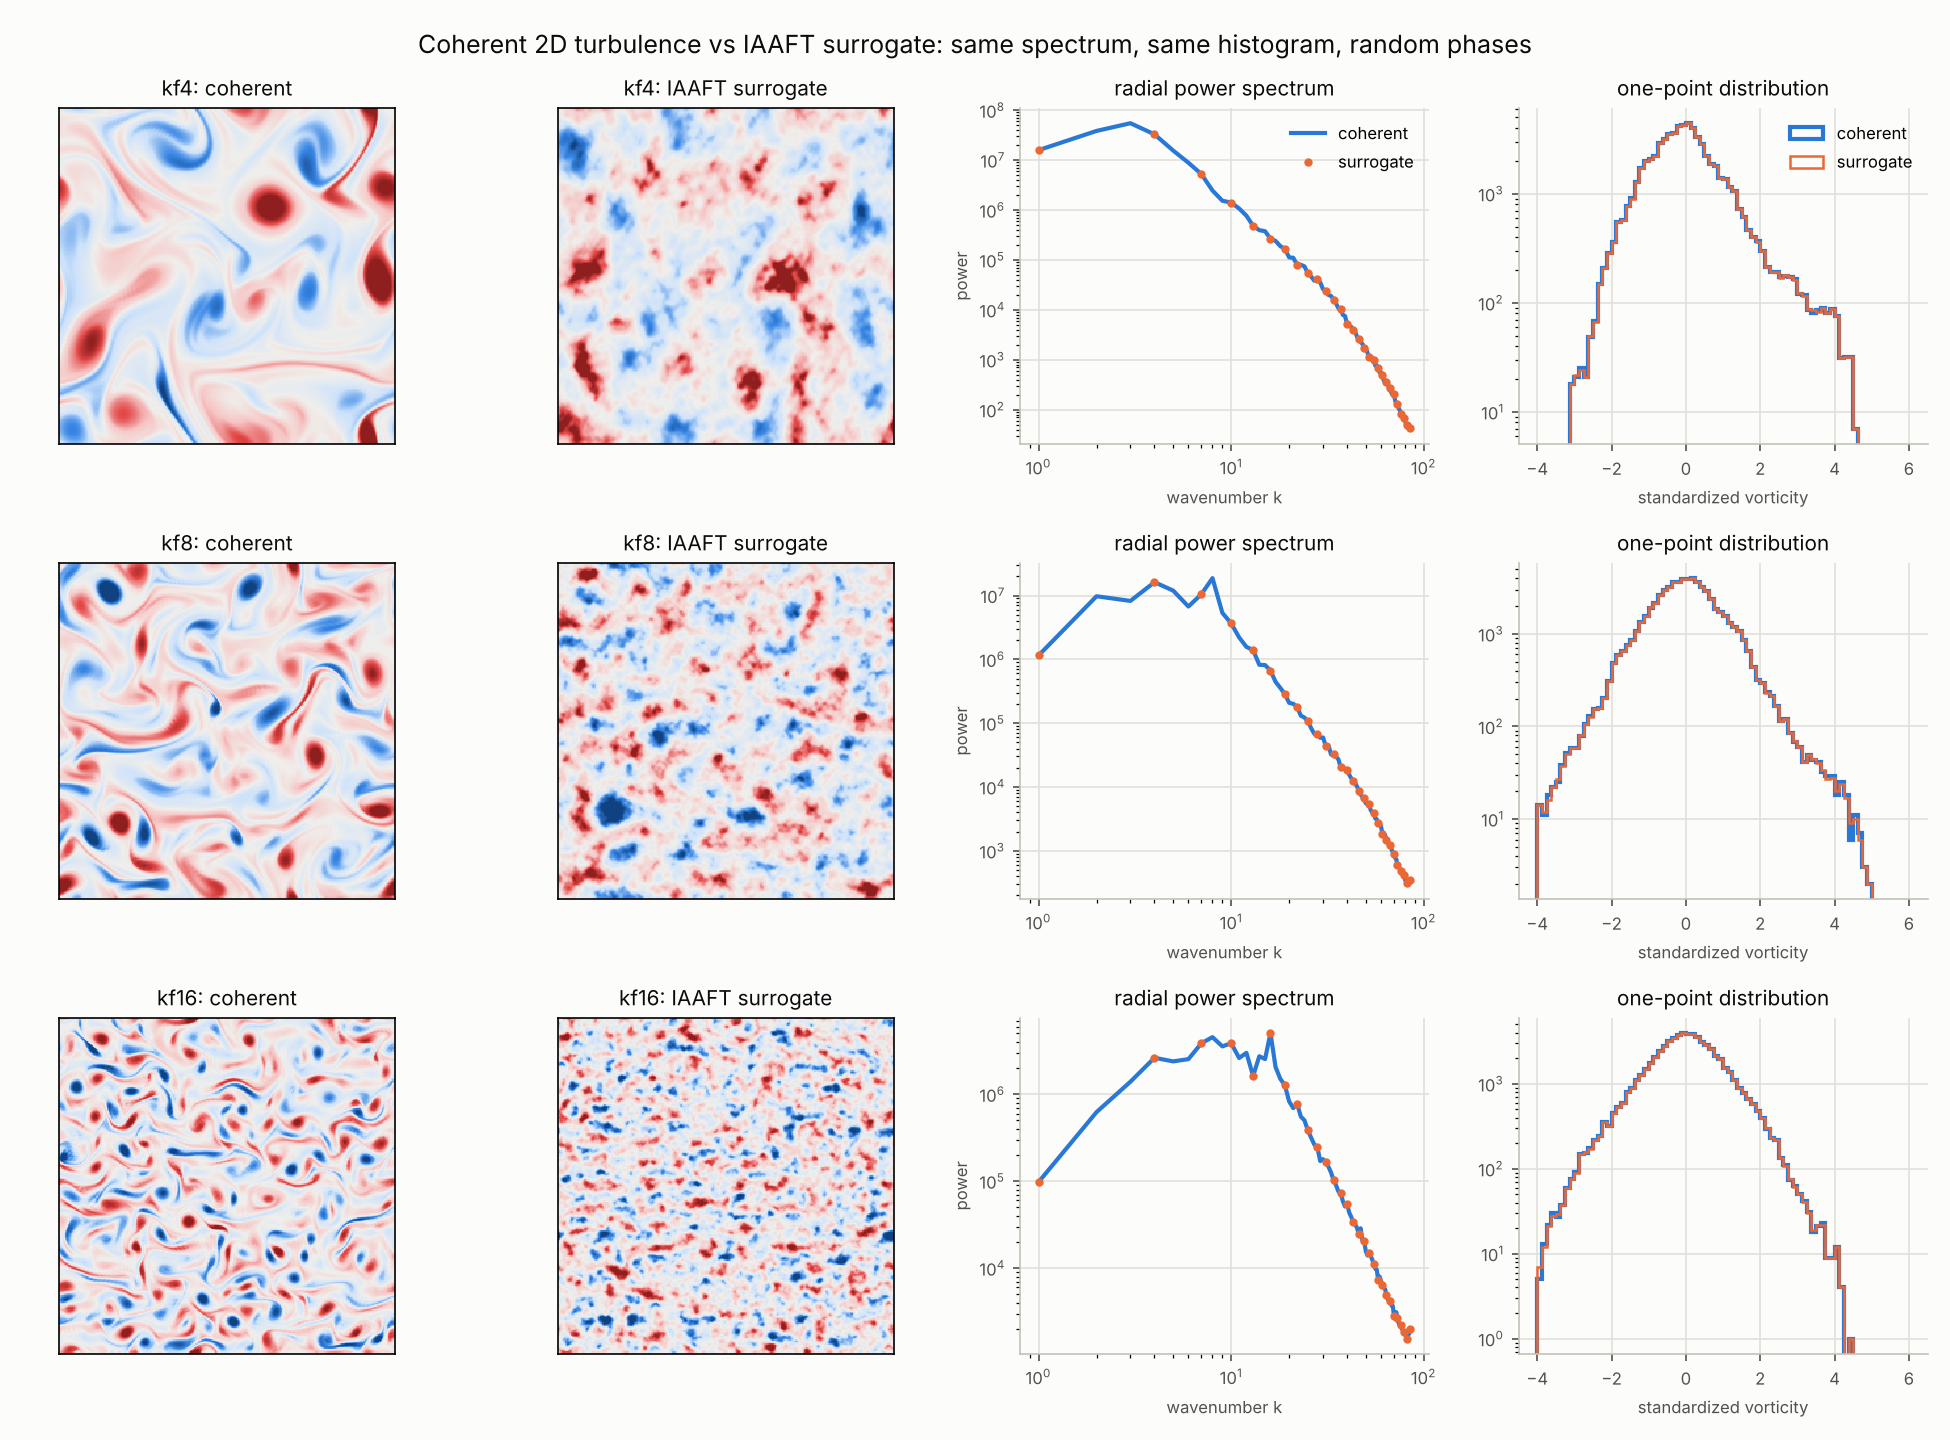
\includegraphics[width=\textwidth]{fields_coherent_vs_iaaft.png}
\caption{One snapshot per forcing scale (rows). Left to right: standardized
vorticity, its IAAFT surrogate, and their radial power spectra and one-point
distributions, which coincide.}
\label{fig:fields}
\end{figure}

\section{Descriptors, baselines and protocol}

\paragraph{Topological and multiview features.} The \emph{topological view}
computes the sublevel-set persistent homology of the cubical complex of the
field \cite{gudhi}. The image is down-sampled to $64^2$, and the $H_0$ and
$H_1$ diagrams are summarized by their count, total and maximal persistence
and persistence entropy (8 numbers). The \emph{spectral view} contains the
spectral slope, the log total power, the spectral peak and the 8 smallest
eigenvalues of the normalized Laplacian of a $16^2$ grid graph weighted by
vorticity similarity. The \emph{descriptor} concatenates
the two views. All three were fixed before any run. Afterwards we tested
richer vectorizations of the same filtration, all with fixed
hyper-parameters, which therefore cannot be fitted across folds:
\begin{itemize}
\item persistence images \cite{adams2017}, 2 images of $10\times10$ pixels, on the $256^2$ field;
\item Betti curves $\beta_0(t)$ and $\beta_1(t)$ at 33 thresholds;
\item a multi-scale filtration: persistence of the field after a periodic
  Gaussian low-pass with $\sigma=1,2,4,8$ grid cells, with 16 summaries per
  scale.
\end{itemize}
We also tested the two views of the reference multiview implementation
\cite{multiview}. The functional-graph view X1 consists of 10 invariants of
the graph of $8\times8$ regions linked when $|\mathrm{corr}|>0.4$. The
persistence view X2 has 12 summaries of the periodic sublevel filtration at
$256^2$.

\paragraph{Baselines.} The baselines fall into three groups:
\begin{itemize}
\item \emph{Blind by construction}: spectral slope, the full log radial
  spectrum (85 bins), vorticity moments and 19 one-point quantiles. The full
  spectrum and the quantiles serve as leak detectors.
\item \emph{Raw pixels}: a $16\times16$ down-sampled image.
\item \emph{Classical coherent-structure diagnostics}, which are phase-sensitive
  but involve no topology:
  \begin{itemize}
  \item statistics of the Okubo--Weiss parameter
    $W=s_n^2+s_s^2-\omega^2$, with $s_n=u_x-v_y$ and $s_s=v_x+u_y$,
    including the vortex-core fraction $W<-0.2\,\sigma_W$
    \cite{okubo1970,weiss1991,isern2006};
  \item skewness and flatness of $|\nabla\omega|$ and $\nabla^2\omega$,
    flatness of $\partial_x\omega$ and $\partial_y\omega$, and the
    correlation of $\omega^2$ with $|\nabla\omega|^2$ (7 numbers);
  \item the flatness of vorticity increments,
    $F(r)=\langle\delta_r\omega^4\rangle/\langle\delta_r\omega^2\rangle^2$,
    for $r\in\{1,2,4,8,16,32\}$ cells along $x$ and $y$.
  \end{itemize}
\end{itemize}
The variances of these derivative and increment fields are fixed by the
spectrum, but their higher moments are not. The reference baseline $B_\cup$ concatenates every non-topological baseline
except raw pixels (136 numbers).

\paragraph{Protocol.} We use repeated StratifiedGroupKFold cross-validation
(4 folds $\times$ 5 repeats). The group is the trajectory, so a snapshot, its
surrogate and every correlated snapshot of the same run always share a fold.
The classifiers are logistic regression and a random forest with 300 trees
\cite{sklearn}, and for every feature set we report the better of the two.
We give 95\% confidence intervals for accuracy differences from a paired
bootstrap over trajectories (2000 resamples). The decision rule was fixed in
advance: a configuration counts as better only if it beats $B_\cup$ by at
least $+0.05$ accuracy.

\section{Results}

\begin{table}[t]
\centering
\small
\begin{tabular}{lrcc}
\toprule
Feature set & dim & binary (primary) & 6 classes \\
\midrule
\multicolumn{4}{l}{\emph{Blind by construction / leak detectors}}\\
spectral slope & 1 & 0.500 & 0.500 \\
full log power spectrum & 85 & 0.500 & 0.500 \\
one-point quantiles & 19 & 0.503 & 0.425 \\
moments & 6 & 0.500 & 0.334 \\
raw pixels ($16\times16$) & 256 & 0.782 & 0.601 \\
\midrule
\multicolumn{4}{l}{\emph{Classical coherent-structure diagnostics}}\\
Okubo--Weiss statistics & 6 & 0.974 & 0.791 \\
gradient / Laplacian statistics & 7 & \textbf{1.000} & 0.800 \\
increment flatness & 12 & 0.976 & 0.830 \\
all non-topological, $B_\cup$ & 136 & 0.999 & \textbf{0.998} \\
\midrule
\multicolumn{4}{l}{\emph{Topological and multiview}}\\
spectral view & 11 & 0.580 & 0.571 \\
topological view ($64^2$, pre-registered) & 8 & 0.983 & 0.982 \\
descriptor (spectral + topological) & 19 & 0.989 & 0.991 \\
topological view at $256^2$ & 8 & 1.000 & 1.000 \\
persistence images & 200 & 0.993 & 0.997 \\
Betti curves & 66 & 0.988 & 0.991 \\
multi-scale filtration & 64 & 1.000 & 1.000 \\
X1 functional graph & 10 & 0.692 & 0.720 \\
X2 persistence summaries & 12 & 1.000 & 1.000 \\
\bottomrule
\end{tabular}
\caption{Accuracy under trajectory-grouped cross-validation on clean fields
(chance: 0.500 binary, 0.167 for 6 classes). The headroom over $B_\cup$ is at
most 0.002 on these two tasks and at most 0.011 on the per-scale tasks.}
\label{tab:main}
\end{table}

\paragraph{The benchmark is structure-only.} The spectrum and quantile
classifiers sit at chance (Table~\ref{tab:main}), so neither the spectrum nor
the one-point distribution separates the classes. Raw pixels reach only 0.78:
480 samples are too few to learn translation-invariant structure.

\paragraph{Topology detects structure, but so do classical diagnostics.} Eight
persistence summaries of a coarse $64^2$ filtration separate coherent fields
from their surrogates with 98.3\% accuracy, and 100\% at full resolution. The
spectral view is near chance, so the descriptor's 98.9\% comes from topology.
A 7-number vector of gradient statistics reaches 100\%, however, and
Okubo--Weiss statistics and increment flatness reach about 97.5\%. Against the
strongest baseline, the descriptor's margin on the primary task is $-0.011$
(95\% CI $[-0.018,-0.005]$). Within each forcing scale the best topological
and the best classical feature sets both reach 1.000. Richer vectorizations (persistence images,
Betti curves, the multi-scale filtration) and the full multiview descriptor
X1+X2 all reach 0.99--1.00. Across all configurations and tasks no margin
over $B_\cup$ has a CI lower bound above 0, and the largest point margin is
$+0.011$. Adding topology to $B_\cup$ changes accuracy by at most $+0.011$.
Two further observations:
\begin{itemize}
\item The gain over the pre-registered view comes from resolution, not from
  vectorization. The plain 8 summaries at $256^2$ already score 1.000.
\item The one large win, topology over the classical diagnostics alone in the
  6-class task (0.982 vs 0.926), reflects scale information. Persistence
  counts grow with $k_f$, while the classical diagnostics are scale-free.
  The win disappears once spectral baselines are added ($B_\cup$, 0.998).
\end{itemize}

\paragraph{Degraded fields.} A pre-registered study applied five degradation
models at four levels each, identically to both classes: white noise,
random missing pixels, contiguous gaps, quantization and resolution loss.
Benjamini--Hochberg correction was applied over 552 comparisons. Besides
$B_\cup$, every topological configuration was compared with a
\emph{matched-scale control}: the same classical diagnostics computed on the
same Gaussian pyramid as the multi-scale filtration. The results
(Table~\ref{tab:degraded}, Fig.~\ref{fig:noise}) are:
\begin{itemize}
\item Single-scale persistence degrades sharply under noise. X2 drops to 0.80
  at 0\,dB SNR and 0.59 at $-5$\,dB. So do the gradient statistics (0.59 and
  0.50).
\item The multi-scale filtration stays at 0.99. At $-5$\,dB this gives the
  only significant advantage over $B_\cup$ anywhere in the study ($+0.287$,
  CI $[+0.253,+0.322]$).
\item The matched-scale control reaches 0.998 at $-5$\,dB, so the advantage
  comes from smoothing, not from topology.
\item Missing data and quantization leave no headroom ($B_\cup\ge0.995$).
  Strong resolution loss hurts topology more than the baselines ($-0.139$ at
  $\times16$).
\end{itemize}

\begin{table}[t]
\centering
\small
\begin{tabular}{lccccc}
\toprule
Condition & multi-scale & $B_\cup$ & matched-scale & margin vs $B_\cup$ & margin vs control \\
 & topology & & control & [95\% CI] & [95\% CI] \\
\midrule
clean & 1.000 & 1.000 & 1.000 & $+0.000$ & $+0.000$ \\
noise 0\,dB & 0.995 & 0.956 & 1.000 & $+0.039\ [+0.018,+0.065]$ & $-0.005\ [-0.011,+0.000]$ \\
noise $-5$\,dB & 0.992 & 0.706 & 0.998 & $+0.287\ [+0.253,+0.322]$ & $-0.006\ [-0.017,+0.004]$ \\
resolution $\times16$ & 0.719 & 0.858 & 0.868 & $-0.139\ [-0.176,-0.101]$ & $-0.149\ [-0.185,-0.112]$ \\
\bottomrule
\end{tabular}
\caption{Binary task under degradation (4 folds $\times$ 3 repeats). The
matched-scale control is $B_\cup$ plus the classical diagnostics on the
multi-scale filtration's own Gaussian pyramid ($\sigma=1,2,4,8$).}
\label{tab:degraded}
\end{table}

\begin{figure}[t]
\centering
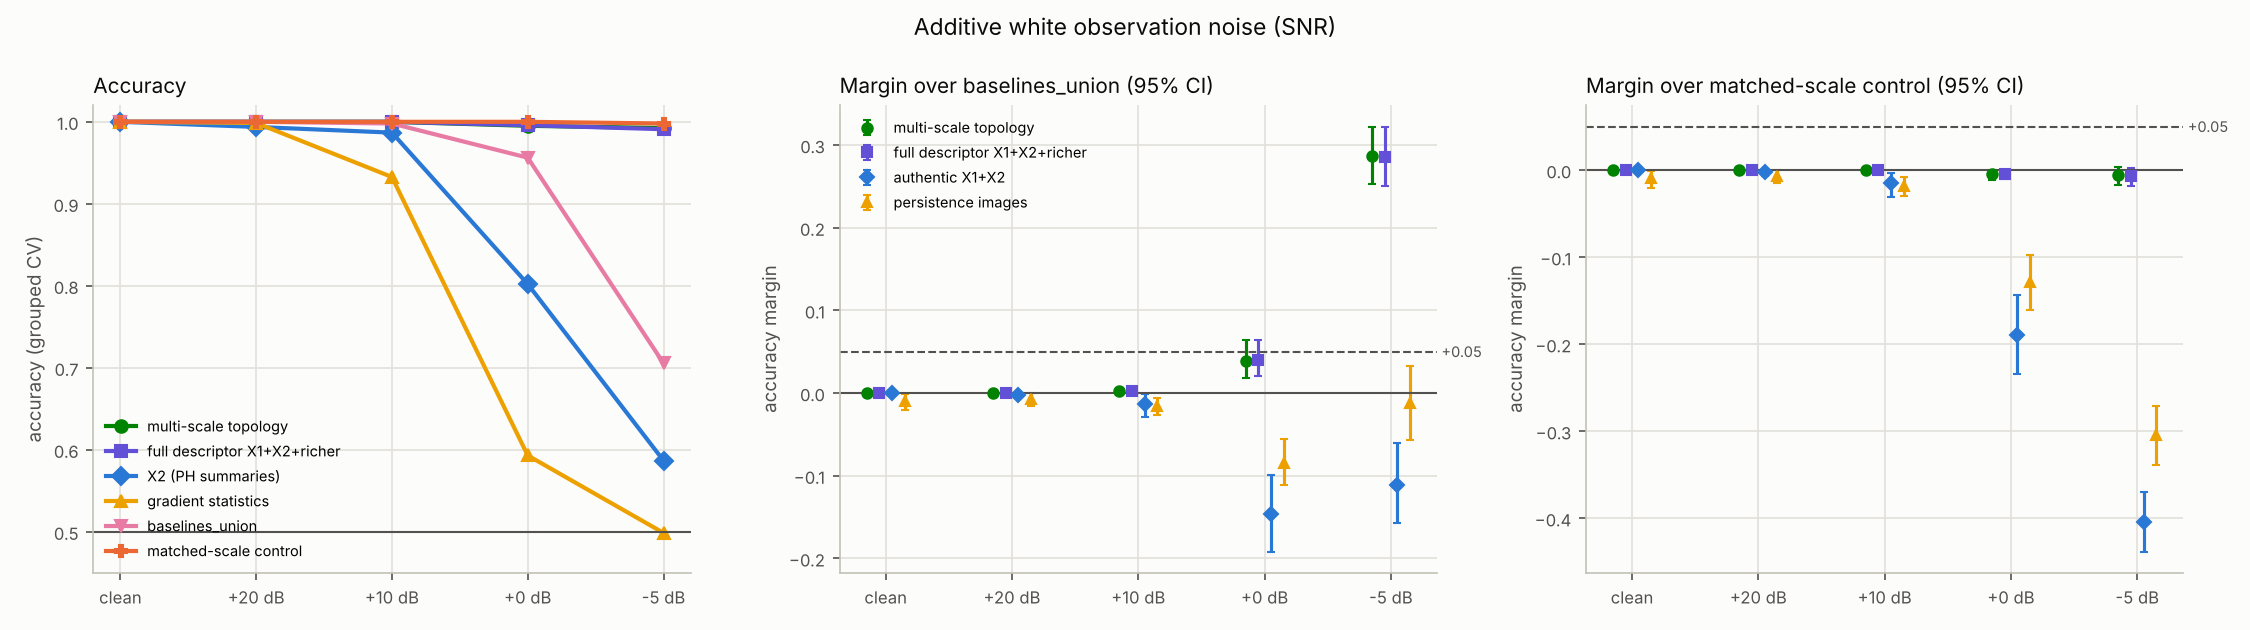
\includegraphics[width=\textwidth]{robustness_noise.png}
\caption{Additive white observation noise. Left: accuracy. Centre: margin of
topological configurations over $B_\cup$. Right: margin over the
matched-scale control. The dashed line is the $+0.05$ decision threshold.}
\label{fig:noise}
\end{figure}

\paragraph{A standardization pitfall.} Standardizing a field as
$(\omega-m)/(s+\varepsilon)$ yields a standard deviation of
$1-\varepsilon/s$. This encodes the original amplitude $s$ at round-off level,
and feature scaling inside the classifier amplifies it. In our pipeline this
alone let vorticity moments separate coherent fields from histogram-identical
surrogates perfectly (accuracy 1.000), until the $\varepsilon$ was removed
and all features were rounded to $10^{-8}$. Benchmarks that "remove
amplitude" by standardization should check for this leak.

\section{Discussion and conclusion}

The coherent-versus-surrogate task is a nonlinearity test in the sense of
\cite{theiler1992}. Any statistic that depends on Fourier phases can pass it,
and the local derivative- and increment-based diagnostics of 2D turbulence
already do so almost perfectly. Persistent homology captures the same
structure, robustly and with few numbers, but on this benchmark it adds no
measurable information beyond those diagnostics. This holds for every
vectorization we tried and for the full multiview descriptor. Its apparent
advantages trace back to resolution, scale information or built-in smoothing,
and each disappears under a like-for-like control. We draw two
methodological lessons for topological flow descriptors:
\begin{itemize}
\item Benchmarks should remove spectral and one-point shortcuts and report
  leak detectors.
\item Baselines should include the classical diagnostics of the field and
  receive the same preprocessing (resolution, smoothing, scales) as the
  topology.
\end{itemize}

\paragraph{Limitations and outlook.} The study is limited to synthetic data
from a single flow family. On it, the strongest baselines leave at most
$0.011$ accuracy of headroom on clean fields, so no descriptor could show a
$0.05$ advantage there. Classical diagnostics are local, whereas topology is
sensitive to the connectivity of large-scale patterns. A natural next test is
therefore a task decided by that connectivity, such as atmospheric blocking
versus zonal flow in reanalysis data \cite{tibaldi1990,davini2012}. A
pipeline for ERA5 500\,hPa fields is prepared but has not been run.

\paragraph{Code and data availability.} The solver, IAAFT surrogates,
descriptors, baselines, configurations (with fixed seeds) and all result
tables are available at
\url{https://github.com/Dcrr1717/gem-geophysical-descriptor}.
% TODO: archive a release and cite its DOI.

\begin{thebibliography}{99}\small

\bibitem{adams2017} H.~Adams, T.~Emerson, M.~Kirby, R.~Neville, C.~Peterson,
P.~Shipman, S.~Chepushtanova, E.~Hanson, F.~Motta, L.~Ziegelmeier,
Persistence images: a stable vector representation of persistent homology,
\emph{J.\ Mach.\ Learn.\ Res.} 18(8) (2017) 1--35.

\bibitem{cohensteiner2007} D.~Cohen-Steiner, H.~Edelsbrunner, J.~Harer,
Stability of persistence diagrams, \emph{Discrete Comput.\ Geom.} 37 (2007)
103--120.

\bibitem{davini2012} P.~Davini, C.~Cagnazzo, S.~Gualdi, A.~Navarra,
Bidimensional diagnostics, variability, and trends of Northern Hemisphere
blocking, \emph{J.\ Climate} 25 (2012) 6496--6509.

\bibitem{edelsbrunner2010} H.~Edelsbrunner, J.~Harer, \emph{Computational
Topology: An Introduction}, American Mathematical Society, Providence, 2010.

\bibitem{gudhi} The GUDHI Project, \emph{GUDHI User and Reference Manual},
GUDHI Editorial Board, \url{https://gudhi.inria.fr}.

\bibitem{isern2006} J.~Isern-Fontanet, E.~Garc\'ia-Ladona, J.~Font, Vortices
of the Mediterranean Sea: an altimetric perspective, \emph{J.\ Phys.\
Oceanogr.} 36 (2006) 87--103.

\bibitem{kramar2016} M.~Kram\'ar, R.~Levanger, J.~Tithof, B.~Suri, M.~Xu,
M.~Paul, M.~F.~Schatz, K.~Mischaikow, Analysis of Kolmogorov flow and
Rayleigh--B\'enard convection using persistent homology, \emph{Physica D} 334
(2016) 82--98.

\bibitem{multiview} [Authors -- TODO], Topological--spectral multiview
descriptor for neural-architecture discrimination, PanAm 2026, EPN Quito.
Reference implementation:
\url{https://github.com/Dcrr1717/multiview-nn-descriptor}. % TODO: complete

\bibitem{okubo1970} A.~Okubo, Horizontal dispersion of floatable particles in
the vicinity of velocity singularities such as convergences, \emph{Deep-Sea
Res.} 17 (1970) 445--454.

\bibitem{sklearn} F.~Pedregosa et al., Scikit-learn: machine learning in
Python, \emph{J.\ Mach.\ Learn.\ Res.} 12 (2011) 2825--2830.

\bibitem{schreiber1996} T.~Schreiber, A.~Schmitz, Improved surrogate data for
nonlinearity tests, \emph{Phys.\ Rev.\ Lett.} 77 (1996) 635--638.

\bibitem{theiler1992} J.~Theiler, S.~Eubank, A.~Longtin, B.~Galdrikian,
J.~D.~Farmer, Testing for nonlinearity in time series: the method of
surrogate data, \emph{Physica D} 58 (1992) 77--94.

\bibitem{tibaldi1990} S.~Tibaldi, F.~Molteni, On the operational
predictability of blocking, \emph{Tellus A} 42 (1990) 343--365.

\bibitem{venema2006} V.~Venema, F.~Ament, C.~Simmer, A stochastic iterative
amplitude adjusted Fourier transform algorithm with improved accuracy,
\emph{Nonlin.\ Processes Geophys.} 13 (2006) 321--328.

\bibitem{weiss1991} J.~Weiss, The dynamics of enstrophy transfer in
two-dimensional hydrodynamics, \emph{Physica D} 48 (1991) 273--294.

\end{thebibliography}
\end{document}
